\graphicspath{{img/metodos/}}
\chapter{Métodos Numéricos}

\section*{Presentación}

Una amplia gama de problemas de ingeniería se reducen a la solución de un 
sistema de ecuaciones diferenciales que gobiernan el comportamiento
de una región del espacio de alguna función de interés. Para que exista alguna 
posibilidad de solución la región de interés debe estar además limitada por una 
superficie (o frontera) sobre la cual se deben conocer además algunas 
características de la solución. En matemáticas, este tipo de formulaciones se 
conocen como problemas de contorno o de valores en la frontera (PVF), y si 
además involucran variaciones en el tiempo entonces se denominan problemas de 
valores iniciales y en la frontera (PVI-F).

Sin embargo, en la mayoría de casos reales la solución de los problemas de
valores en la frontera es imposible de conseguir por medio de métodos 
analíticos que produzcan soluciones cerradas, es decir funciones. Como 
alternativa de solución aparece la posibilidad de recurrir a planteamientos 
matemáticos que permiten re-escribir los PVF en términos de formulaciones muy 
amigables para ser resueltas en el computador. En el caso de problemas de 
ingeniería con una base mecánica como mecánica de suelos, mecánica de sólidos, 
y mecánica de fluidos, los PVF asociados suelen resolverse por métodos que 
forman la base de la denominada Mecánica Computacional. Por ejemplo los métodos 
de desplazamientos y fuerzas utilizados para el análisis de edificios y otras 
estructuras, pertenecen a la mecánica computacional. Similarmente, en la 
solución de problemas más complejos se usan los métodos de elementos finitos 
(FEM por sus siglas en ingles), los métodos de diferencias finitas (FDM por sus 
siglas en ingles) y el método de elementos de frontera (BEM por sus siglas en 
ingles).

En este capítulo revisamos de manera practica algunas técnicas numéricas que 
son fundamentales en la formulación de métodos típicos de la Mecánica 
Computacional como los ya descritos. En particular, estaremos cubriendo los 
siguientes métodos:
,\begin{itemize}
\item Solución de ecuaciones no lineales (determinación de raíces)

\item Interpolación

\item Integración numérica
\end{itemize}

Al final de este capitulo el estudiante estará en la capacidad de:
\begin{itemize}
\item Reconocer el concepto de raíz de una función (o conjunto de funciones) y 
manejar los métodos básicos para su determinación en funciones escalares de una 
variable.

\item Resolver manualmente o con la ayuda de implementaciones en el 
computador problemas de determinación de raíces.

\item Reconocer el problema de interpolación como uno de aproximación de 
funciones que originalmente se desconocen en forma cerrada.

\item Manejar los aspectos matemáticos fundamentales del método de 
interpolación de Lagrange.

\item Resolver manualmente o con la ayuda de implementaciones en el 
computador problemas de aproximación de funciones a través de métodos de 
interpolación.

\item Reconocer los principios matemáticos básicos del problema de integración 
numérica de funciones sobre dominios en una y dos dimensiones.

\item Resolver manualmente o con la ayuda de implementaciones en el 
computador problemas de calculo numérico de integrales de funciones.
\end{itemize}


\section{Raíces de Ecuaciones}
El problema de determinación de raíces (o de los ceros) de una función se 
presenta frecuentemente en diferentes aplicaciones de ingeniería y física. Acá 
discutiremos 2 métodos que pueden considerarse clásicos, como son el método de 
bisección y el método de Newton-Raphson. El primero tiene valor ya que es 
bastante intuitivo aunque no siempre eficaz, mientras que el segundo, al 
desprenderse de la expansión de una función en su serie de Taylor permite 
generalizarse a problemas de sistemas de ecuaciones.

\subsection{Planteamiento del problema}

Consideremos una función escrita de la forma
\begin{equation}
y=f(x)
\label{funcionY}
\end{equation}

la cual seguramente sabemos interpretar como una regla que transforma valores
de la variable independiente $x$ en valores de la variable dependiente $y$ y
donde $f(x)$ es la regla de la transformación, ver \cref{fig:ecuacion}.

\begin{figure}[H]
	\centering
	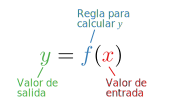
\includegraphics[width=50 mm]{ecuacion.pdf}
	\caption{Descripción del concepto de función como una regla de
	transformación de valores (posiblemente) reales  en otros valores
	(posiblemente) reales.}
	\label{fig:ecuacion}
\end{figure}

Por ejemplo, un caso particular de una regla de transformación o función puede 
ser de la forma:
\[f(x) = \ x^3 + 4x^2 - 10\, .\]

El problema de búsqueda de raíces de la función consiste en encontrar valores 
de la variable independiente $x$ que cuando sean transformados por la regla 
$f(x)$ produzcan valores nulos de $y$. Matemáticamente esta pregunta la podemos 
plantear como encontrar valores de $x$ que satisfagan la condición:
\[f(x) = 0.0\, .\]

Por ejemplo, la \cref{fig:raiz} muestra la variación de la función
\[f(x) = \ x^3 + 4x^2 - 10\, ,\]
para valores de $x$ en el intervalo $[-4, 2].$ En la gráfica el círculo blanco 
correspondiente a la intersección de la línea $y=0$ y la función corresponde a 
una raíz de la función. Esta tiene un valor aproximado de $x=1.4.$

\begin{figure}[H]
	\centering
	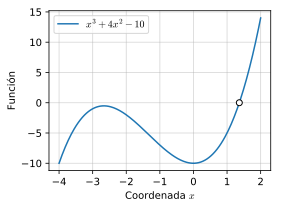
\includegraphics[width=4 in]{raiz.pdf}
	\caption{Concepto de raíz de una función. La función sobre el intervalo
	$[-4.0, 2.0]$ se muestra con la línea azul y la raíz con el círculo blanco.}
	\label{fig:raiz}
\end{figure}


La función puede tener varias raíces reales (positivas o negativas) o inclusive
varias raíces complejas.

\paragraph{Ejemplo: Determinación de caudal.}
Un problema típico en ingeniería hidráulica es el de determinar el caudal $Q$ 
con el que es necesario alimentar una turbo-máquina de potencia especifica
$\phi$, resistencia total a fluir $R_T$ la cual está localizada entre 2 niveles 
con salto $\Delta H$. Usando argumentos de conservación de energía se puede 
demostrar que este caudal satisface la condición:

\begin{equation}
	{R_T}{Q^3} - \Delta HQ + \phi  = 0.
\label{caudal}
\end{equation}

Claramente, se trata de un problema de determinación de raíces tras encontrar 
el caudal $Q$ que satisfaga la condición:
\[f(Q) = 0.0\, ,\]
donde
\begin{equation}
f(Q) ={R_T}{Q^3} - \Delta HQ + \phi\, .
\label{caudalF}
\end{equation}

\begin{tcolorbox}
En computación se denomina \textbf{iteración} un procedimiento que se aplica al 
resultado de una operación previa.
\end{tcolorbox}

En general, los métodos de determinación de raíces son iterativos y requieren 
de una estimación inicial de la raíz (o raíces). De acuerdo con dicha 
estimación se pueden tener los siguientes resultados (ver 
\cref{fig:raizconverge}):
\begin{itemize}
	\item Falla de convergencia.
	\item Convergencia a un valor incorrecto.
	\item Convergencia a un valor correcto.
\end{itemize}

Antes de iniciar el estudio de un par de métodos clásicos para 
determinación de raíces es importante tener una idea de los conceptos de 
convergencia y divergencia. Intuitivamente, decimos que un método converge 
cuando los valores se acercan cada vez más y que diverge cuando pasa lo 
contrario, se alejan entre ellos. Adicionalmente, llamamos \textbf{tasa de 
convergencia} a la rapidez con la que un cálculo iterativo se aproxima a una 
solución. Ahora, concentrémonos en la \cref{fig:raizconverge} en la cual se 
grafica la variación del error vs el número de iteraciones en un algoritmo. 
La gráfica presenta el porcentaje de error contra el número de iteraciones 
requeridas para predecir la raíz $x=1.3652305$ por medio de los 2 métodos que 
estudiaremos en esta sección a saber el método de bisección y el método de 
Newton. Podemos ver que uno de los métodos converge más rápidamente que el otro.

\begin{figure}[H]
  \centering
  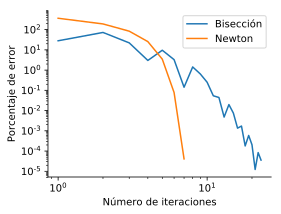
\includegraphics[width=4 in]{convergencia.pdf}
  \caption{Concepto de convergencia o número de iteraciones requeridas para
  alcanzar una solución.}
  \label{fig:raizconverge}
\end{figure}
	

\subsection{Localización incremental de raíces}

El cálculo de las raíces de una ecuación involucra 2 procesos que se discutirán 
a continuación. Inicialmente se identifican de manera aproximada las 
localizaciones de las raíces en un intervalo determinado. Este proceso se 
denomina \textbf{detección} o \textbf{bracketing}. El proceso de detección 
arroja valores de las raíces con baja precisión.

Para mejorar la precisión se ejecuta un segundo paso tras seleccionar una 
precisión especificada mediante una \textbf{tolerancia} o valor de referencia. 
La tolerancia indica cual es la definición aceptable de cero para determinar si 
efectivamente se encontró la raíz. Esta es necesaria ya que en el computador 
solo es posible especificar el cero hasta cierto número de cifras 
significativas, en otras palabras, en el computador no existe el cero 
matemático. El segundo proceso corresponde entonces al acercamiento a la raíz 
con una precisión dada y definida en términos de la tolerancia. Este segundo 
paso se denomina \textbf{determinación} de la raíz. En resumen, el 
proceso de búsqueda de raíces implica 2 pasos:

\begin{itemize}
	\item[i.] Localización inicial de las raíces o {\bf Detección}.
	\item[ii.] Acercamiento o mejoramiento en la precisión del valor de la
	raíz o {\bf Determinación}.
\end{itemize}

En el proceso de detección de la raíz la idea fundamental consiste en recorrer 
la función por intervalos de tamaño $\Delta x$ y con límites $x_1$ y $x_2$. Si 
durante el recorrido se encuentra que los valores $f(x_1)$ y $f(x_2)$ de las 
funciones tienen signos diferentes, entonces se concluye que existe al menos 
una raíz en el intervalo. El proceso se resume en los siguientes 2 pasos:

\begin{itemize}
	\item[i]  Recorrido del dominio por intervalos $\Delta x$.
	\item[ii] Evaluación de la función para detectar cambios de signo.
\end{itemize}

Para explicar el proceso y su eventual solución en el computador tomemos como 
referencia la \cref{fig:bracketing} en la que se presenta una función que tiene 
2 raíces (círculos negros) en el intervalo $[a,b]$. El proceso de detección se 
describe además en el \cref{alg:brack}. Los datos de entrada al problema son 
los extremos del intervalo correspondientes a $x=a$ y $x=b$; el número de 
subintervalos $N$ en los que se partirá el dominio del problema; y la función 
$f(x)$ cuya raíz se desea determinar.  El algoritmo entregará como resultado 
las raíces encontradas, las cuales almacenará en un vector denominado $x_R$. En 
el primer paso del algoritmo calculamos el tamaño del subintervalo $\Delta x$ y 
fijamos el contador de detección de raíces $iroot$ en cero. Este contador se 
incrementará en 1 cada que el algoritmo detecte una raíz.

La parte principal del algoritmo consiste en un ciclo que recorre los $N$ 
subintervalos en los que se ha partido el problema y detecta cambios de signo 
haciendo evaluaciones del producto $f (x_1) \times f (x_2).$ Si se da la 
condición $f \left( x_1 \right) \times f \left( x_2 \right) < 0.0$ entonces se 
concluye que existe una raíz en algún punto entre $x=x_1$ y $x=x_1+ \Delta x$. 
Este evento queda registrado en el contador $iroot$. Al mismo tiempo se 
selecciona el inicio del intervalo como el de localización aproximada de la 
raíz. Esta se almacena en la posición $irrot$ del vector $x_R$ . Este algoritmo 
sencillo se da como referencia en el apéndice de estas notas.

\begin{figure}[H]
\centering
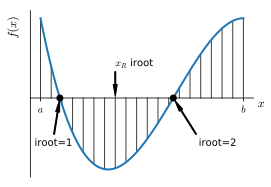
\includegraphics[width=4 in]{busquedas_inc.pdf}
\caption{Proceso de detección de raíces de una función en un intervalo $[a,b]$.}
\label{fig:bracketing}
\end{figure}


\begin{algorithm}[H]
\SetAlgoLined
\KwData{$a, \ b, \ N, \ f$}
\KwResult{$x_R$: Vector con la aproximación de las raíces}
\BlankLine

$\Delta x \leftarrow \dfrac{b - a}{N - 1}$;\\
\BlankLine
$iroot \leftarrow 0$ ;\\
\BlankLine
$x_2 \leftarrow a$ ;\\
\BlankLine
\For{$i \leftarrow 0$ to $N - 1$}{
	$x_1 \leftarrow x_2$;\\
	$x_2 \leftarrow x_1+\Delta x$;\\
	\If{$f (x_1) \times f (x_2) <0.0$}{
		$iroot \leftarrow iroot+1$;\\
		$x_R [i] \leftarrow x_1$;\\
		}
	\BlankLine
	}
\BlankLine
\caption{Detección o \textit{bracketing}.}
\label{alg:brack}
%
\end{algorithm}

La aplicación del código anterior a la función $f(x) = \ x^3 + 4x^2 - 10$ en el 
intervalo comprendido entre $a=-10.0$ y $b=10.0$ con $\Delta x = 1.0$ produce 
el vector de raíces $x_R$
\begin{verbatim}
A change of sign was found.
[0. 0. 0. 0. 0. 0. 0. 0. 0. 0. 0. 1. 0. 0. 0. 0. 0. 0. 0. 0. 0.]
\end{verbatim}
el cual indica que la función tiene un cero en el intervalo $[1.0,2.0]$ y 
localizado aproximadamente en $x = 1.0$. Este valor de la raíz debe ser 
posteriormente refinado para encontrar el valor consistente con la tolerancia 
prescrita. En las secciones que se presentan a continuación discutiremos 2 
métodos clásicos usados para realizar este refinamiento de la raíz.


\subsection{Método de bisección}
En este paso se asume que ya se ha encerrado una raíz de $f(x) = \ 0.0$ en el intervalo $(x_1, x_2)$ mediante un proceso previo de detección.  Tal y como se describe en la \cref{fig:bisection}, la raíz se encuentra en algún punto entre $x_1$ y $x_2$. Mas aún, el algoritmo de detección entrega como localización aproximada de la raíz $x = x_1$. El siguiente paso consiste entonces en acercarse a la raíz con una precisión deseada. El método de bisección consiste en la partición por mitades del intervalo $\Delta x$ en el que se encuentra localizada la raíz alternando entre posiciones de cambio de signo. Cada que se detecta el cambio de signo se redefine el intervalo de la raíz y esta partición continúa hasta que el intervalo se haga lo suficientemente pequeño. El algoritmo localiza inicialmente el punto intermedio ${x_3} = \frac{1}{2}(x_1 + x_2)$ ubicado entre los extremos del intervalo $x_1$ y $x_2$.

\begin{figure}[H]
\centering
\includegraphics[width=4 in]{biseccion.pdf}
\caption{Método de bisección para encontrar las raíces.}
\label{fig:bisection}
\end{figure}

Si $f (x_1) \times f (x_3) < 0.0 $ entonces existe una raíz entre $x_1$ y $x_3$ en cuyo caso se hace $x_2	\leftarrow x_3$ y se calcula un nuevo ${x_3} = \frac{1}{2}({x_1} + {x_2})$ dividiendo a la mitad el intervalo que contiene a la raíz. Si por el contrario se determina que $f (x_1) \times f (x_3) > 0.0 $ entonces la raíz se localiza entre $x_3$ y $x_2$ en cuyo caso se hace $x_1	\leftarrow x_3$ y se calcula un nuevo ${x_3} = \frac{1}{2}({x_1} + {x_2})$ dividiendo nuevamente el intervalo. Este proceso se resume en la siguiente tabla.
\begin{table}[H]
  \centering
  \begin{tabular}{ll}
	Si $f (x_1) \times f (x_3) < 0.0 $\\ & Raíz entre $x_1$ y $x_3$\\ 
	  & $x_2	\leftarrow x_3$ \\
	  & $x_3 \leftarrow \dfrac{1}{2} (x_1 + x_2)$ \\
	  & Calcula $\Delta x \leftarrow x_3-x_1$ \\\\
	Si $f (x_1) \times f (x_3) > 0.0 $\\ & Raíz entre $x_3$ y $x_2$\\ 
      & $x_1	\leftarrow x_3$ \\
      & $x_3 \leftarrow \dfrac{1}{2} (x_1 + x_2)$ \\
      & Calcula $\Delta x \leftarrow x_2-x_3$
  \end{tabular}
\end{table}

El \cref{alg:repeat} presenta el pseudocódigo para el método de bisección.
\begin{algorithm}[h]
\SetAlgoLined
\KwData{$a, \ b, \ tol, \ f$}
\KwResult{$c$: Aproximación de la raíz}
Set $tol$;\\
$n_{\max}  \leftarrow \ceil{\log_2\left(\frac{b - a}{tol}\right)}$ ;\\
\For{cont $\leftarrow 0$ to $n_{\max}$}{
    $c \leftarrow  \frac{1}{2}(a + b)$;\\
	\eIf{$f (a) f (b) < 0.0$}{
		$b \leftarrow c$;\\
		}{
		$a \leftarrow c$;\\
		}
	\BlankLine
	}
\BlankLine
\caption{Bisección}
\label{alg:repeat}
\end{algorithm}

En el apéndice se presenta el código en Python correspondiente al algoritmo de 
bisección el cual arroja el siguiente resultado tras aplicarlo a la función $f 
(x) = \ x^3 + 4x^2 - 10$, sobre el intervalo [-2, 2], usando una tolerancia 
$tol = 10^{-4}$.

\begin{verbatim}
n: 0, x: 0.0
n: 1, x: 1.0
n: 2, x: 1.5
n: 3, x: 1.25
n: 4, x: 1.375
n: 5, x: 1.3125
n: 6, x: 1.34375
n: 7, x: 1.359375
n: 8, x: 1.3671875
n: 9, x: 1.36328125
n: 10, x: 1.365234375
n: 11, x: 1.3642578125
n: 12, x: 1.36474609375
n: 13, x: 1.36499023438
n: 14, x: 1.36511230469
n: 15, x: 1.36517333984
Maximum number of iterations reached.
1.36517333984375
\end{verbatim}

\subsection{Método de Newton-Raphson}

\textcolor{blue}{Este método tiene la desventaja de que requiere, además de la 
evaluación de la función $f(x)$, también la de su primera derivada $f'(x)$.}

El método de Newton-Raphson suele converger más rápido que el método de 
bisección. Esto se debe a que se incluye más información sobre la función en 
las iteraciones, a saber, las derivada. Por la forma que toma la iteración la 
función debe tener un valor diferente de cero para cada aproximación. Como se 
discutió anteriormente las iteraciones se detiene una vez se alcance el cero 
dentro de una tolerancia prescrita.

\subsubsection*{Derivación matemática}
Sea $x_i$ la $i$-ésima\footnote{Por ejemplo, $x_0$ es el valor 
encontrado por el algoritmo de detección.} aproximación a la raíz buscada y $p$ 
el valor refinado de la raíz que se encuentra en la vecindad de 
$x_i$. Escribiendo la función como una serie de Taylor alrededor de $p$ se 
tiene:
\[f(p)=f(x_i)+f'(x_i)(p-x_i)+{(p-x_i)}^2\frac{f''(x_i)}{2!}+...\]

Luego, asumiendo que $f(p)$ es cercano a cero ($f(p)\approx0$) y linealizando 
se tiene:
\[ 0\approx f(x_i)+f'(x_i)(p-x_i) \]
haciendo $x_{i+1}\equiv p$ y re-escribiendo se tiene la expresión
\[x_{i+1}\approx x_i-\frac{f(x_i)}{f'(x_i)}\]
correspondiente a la iteración de Newton-Raphson que permite determinar la raíz 
aproximada  $x_{i+1}$ a partir de la aproximación $x_i$.

\begin{tcolorbox}
Se denomina \textbf{linealización} a la operación de eliminar los términos de 
orden 2 y superiores y retener solo los términos lineales en una expresión. 
La iteración de Newton-Raphson corresponde a la serie de Taylor 
linealizada de la expansión de la función alrededor de la raíz buscada.
\end{tcolorbox}

\subsubsection*{Derivación geométrica}
Geométricamente, el método de Newton-Raphson consiste en extender la recta 
tangente en el punto actual $x_i$ hasta que cruce el cero para luego hacer la 
siguiente aproximación  en la abscisa de dicho punto de cruce. El proceso se 
ilustra en la \cref{fig:newton} en donde se ve que para iniciar las 
iteraciones se requiere una aproximación inicial ($x_0$) a la raíz. Este valor 
inicial es el encontrado mediante el algoritmo de detección discutido 
anteriormente.

Para derivar el método desde una mirada geométrica partiremos del punto $x_i$, 
encontraremos la recta tangente que pasa por el mismo y lo extenderemos hasta 
su cruce con cero, como ya se describió. Usando la ecuación de la pendiente, 
tenemos
\[m = \frac{0 - f(x_i)}{x_{i+1} - x_i}\, ,\]
pero, sabemos que la pendiente es $m = f'(x_i)$, luego
\[f'(x_i) = -\frac{f(x_i)}{x_{i + 1} - x_i}\, ,\]
y si resolvemos esta ecuación para $x_{i +1}$ obtenemos el punto para el cual 
la recta toma el valor de cero. Este será el nuevo punto inicial para repetir 
el proceso y correspondiente a la iteración de Newton-Raphson.
\begin{equation}
  x_{i + 1} = x_i - \frac{f(x_i)}{f'(x_i)}
  \label{eq:iteracion_newton}
\end{equation}

\begin{figure}[H]
\centering
\includegraphics[width=4 in]{newton_iter.pdf}
\caption{Iteración de Newton-Raphson.}
\label{fig:newton}
\end{figure}


 El \cref{alg:newton} presenta el método de Newton para un punto inicial $x$ 
 mientras que su correspondiente código en Python se presenta en los apendices.

\begin{algorithm}[H]
\SetAlgoLined
\KwData{$x, \ tol, \ n_{\max}, \ f, \ f'$}
\KwResult{Raíz aproximada}
\For{cont $\leftarrow  0$ to $n_{\max}$}{
	\If{$|f'(x)| < tol$}{
		Error, división por número cercano a cero.\\
		}
    $x \leftarrow x - \frac{f(x)}{f'(x)}$;\\
	\If{$|f(x)| < tol$}{
		Pare, se llegó al valor deseado.
		}
	}
\BlankLine
\caption{Newton-Raphson}
\label{alg:newton}
\end{algorithm}



Si se aplica el código correspondiente al algoritmo anterior a la función $f (x) = \ x^3 + 4x^2 - 10$ usando una tolerancia $tol = 10^{-8}$ y una estimación inicial de la raíz correspondiente a $x_2=2.0$ de acuerdo al resultado del algoritmo de detección se obtiene el siguiente resultado tras 4 iteraciones.
\begin{verbatim}
n: 0, x: 2.0
n: 1, x: 1.5
n: 2, x: 1.37333333333
n: 3, x: 1.36526201487
(1.3652300139161466, 'Root found with desired accuracy.')
\end{verbatim}

\newpage
\subsubsection{Ejercicios}
\begin{enumerate}

\item \label{ejer:raices-tan} Detectar la localización de las raíces de la función $f(x) = x - \tan x$ (ver \cref{fig:tan}) en el intervalo $[-10.0,10.0]$.
\begin{figure}[h]
\centering
\includegraphics[width=0.65\textwidth]{tan.pdf}
\caption{Función $f(x) = x - \tan x$.}
\label{fig:tan}
\end{figure}

\item \label{ejer:raices-turbo} Se desea determinar el caudal $Q$ con el que es necesario alimentar una turbomáquina que inicialmente está localizada sobre una conducción con una resistencia al flujo ${R_T} = 149$ $\nicefrac{\unit{s}^2}{\unit{m}^5} $, un salto o diferencia de niveles $\Delta H = 500\ \unit{m}$ y una potencia específica $\phi = 2548$ $\nicefrac{\unit{m}^4}{\unit{s}}$. Ajustar los parámetros de manera que el problema tenga solución física.

\item \label{ejer:raices-zapata} En un problema de diseño estructural de cimentaciones se debe determinar la dimensión en planta de una zapata cuadrada de forma tal que no se exceda el esfuerzo admisible sobre la masa de suelo en la cual se va a apoyar. Empleando la teoría de mecánica de sólidos, se puede demostrar que la dimensión de la zapata cuadrada, que no sobrepasa el esfuerzo admisible $(\sigma_\text{adm})$ satisface la siguiente ecuación:

\begin{align}
	H^3 \sigma_\text{adm} - H P \pm 6 (M_1 + M_2) = 0.0
\end{align}

Dónde:

\begin{itemize}
	\item $H:$ Dimensión en planta de la zapata cuadrada.
	\item $\sigma_\text{adm}:$ Esfuerzo admisible.
	\item $P:$ Carga vertical sobre la zapata.
	\item $M_1, \ M_2:$ Momentos flectores al rededor de dos ejes ortogonales.
\end{itemize}

Se desea determinar la dimensión $H$ de la zapata necesaria para no exceder el esfuerzo admisible $\sigma_\text{adm}= 18 \ \unit{tf}/\unit{m}^2$, si la zapata se encuentra sometida a la carga $P=32 \ \unit{tf}$ y los momentos $M_1= 18 \ \unit{tf}\cdot\unit{m}$ y $M_2= 23 \ \unit{tf}\cdot\unit{m}$.

\end{enumerate}

\section{Interpolación}
El problema de aproximación de funciones a través de técnicas de interpolación aparece de manera recurrente en diferentes aplicaciones de ingeniería. Por ejemplo en el ajuste de datos de laboratorio cuando estos son relativamente estables, en la visualización de funciones y en el desarrollo de métodos de solución de problemas de valores en la frontera. La teoría de interpolación es de especial interés en el método de los elementos finitos, en el cual se obtienen valores de los desplazamientos en una serie de puntos y estos se usan, conjuntamente con métodos de interpolación para determinar deformaciones y tensiones. En esta sección se estudiarán los aspectos fundamentales del problema de interpolación de funciones a partir de polinomios de Lagrange. 
\subsection{Planteamiento del problema}

Sea $f(x)$ una función desconocida analiticamente pero con valores conocidos de manera discreta en $n$ puntos $x_1,  x_2, \cdots, x_n$. Queremos conocer (o interpolar) el valor de $f(x)$ en un punto arbitrario  $x \in [x_1, x_n]$ y que es diferente a uno de los $n-$puntos.

El problema de interpolación consiste precisamente en determinar el valor desconocido de $f(x)$ usando los valores conocidos $\left\{f_1,f_2,...,f_n\right\}$. Por ejemplo, tomemos los valores discretos de una función $f(x)$ que se tiene en la \cref{tab:interp_puntos} y que se muestran mediante circulos negros en la \cref{fig:interp_puntos}.

\begin{center}
	\begin{tabular}{rr}
		\hline
		$x$ & $f(x)$ \\
		\hline 
		$-1.0$  & $-7.000$  \\
		$-0.5$  & $-9.125$  \\
		$ 0.00$  & $-10.00$  \\
		$ 0.50$  & $-8.875$  \\
		$ 1.00$  & $-5.000$  \\
		\hline
	\end{tabular}
	\captionof{table}{Valores conocidos de la función $f(x)$.}
	\label{tab:interp_puntos}
\end{center}
%
\begin{figure}[H]
	\centering
	\includegraphics[height=2.5 in]{interp_puntos.pdf}
	\caption{Puntos correspondientes a valores conocidos de una función. Se desea determinar el valor de la función para puntos diferentes a los de medición.}
	\label{fig:interp_puntos}
\end{figure}


Para determinar los valores desconocidos de la función $f(x)$ usando los valores dados $\left\{f_1,f_2,...,f_n\right\}$ el problema se resuelve en dos pasos:

\begin{enumerate}
	\item  Se propone una función de interpolación que pase por los $n$ valores conocidos. Este paso se ilustra mediante la línea punteada de la \cref{fig:interp_continua}. En nuestro caso, propondremos funciones polinomiales.
		
	\item Una vez se disponga de la función de interpolación esta puede ser usada para predecir el valor en puntos arbitrarios. Si se dispone de $n$ datos o valores conocidos de la función es posible proponer un polinomio de interpolación de orden $n-1$. Sin embargo, si se dispone de un número alto de valores conocidos de la función, puede resultar contraproducente el realizar la aproximación usando un polinomio de alto orden.
	
	
		\begin{figure}[H]
		\centering
		\includegraphics[height=2.5 in]{interp_continua.pdf}
		\caption{Polinomio de interpolación usando los $n$-datos. El polinomio resultante es de orden $n-1$.}
		\label{fig:interp_continua}
	\end{figure}
	
	Alternativamente, es posible dividir el dominio del problema en sub-dominios y proceder con interpolaciones locales. Esta alternativa se muestra en la \cref{fig:interp_tramos} en la cual se realiza una interpolación lineal entre pares de puntos.
	\begin{figure}[h]
		\centering
		\includegraphics[height=2.5 in]{interp_tramos.pdf}
		\caption{Función de interpolación  definida por tramos usando pares de puntos para producir polinomios locales de orden $1$.}
		\label{fig:interp_tramos}
	\end{figure}
	
\end{enumerate}

\paragraph*{Ejemplo: Una aplicación en ingeniería civil.}
En este ejemplo se presenta a manera de pregunta un problema típico de interpolación en Ingeniería Civil. En este caso la interpolación requerida es para una fución en el plano. Como veremos de manera formal mas adelante, la solución de este tipo de problemas usa como ingrediente fundamental la solución al problema de interpolación de funciones uni-dimensionales.

La \cref{fig:ram} muestra la distribución de los equipos de registro sísmico que conforman la red acelerográfica de Medellín. Tras la ocurrencia de un evento sísmico cada uno de estos equipos registra el movimiento del terreno en el sitio particular. Dichos movimientos son usados posteriormente para calcular espectros de respuesta para uso en análisis y diseño de estructuras sismo-resistentes.

\begin{figure}[H]
\centering
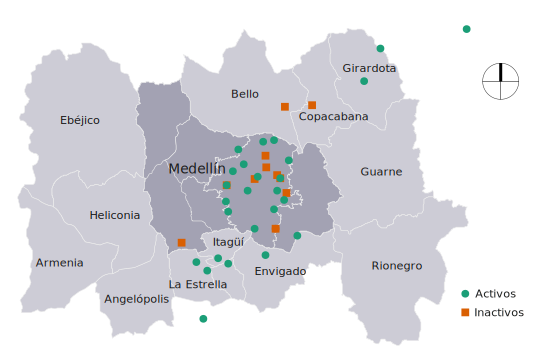
\includegraphics[width=10cm]{red_acelerografica.pdf}
\caption{Red acelerográfica de Medellín. Los círculos verdes representan estaciones activas. Mientras que los cuadrados naranja son estaciones inactivas. Datos de julio de 2017, tomados de SIATA\cite{SIATA_acelerografica}}
\label{fig:ram}
\end{figure}

Como se aprecia en la figura, la cobertura espacial es limitada, lo que dificulta el problema de análisis estructural en zonas de la ciudad donde no se disponga de instrumentación. Se requiere entonces usar una alternativa numérica que permita determinar los espectros de respuesta en sitios carentes de instrumentación de manera consistente con los resultados instrumentales. En términos matemáticos el problema corresponde a uno de interpolación o cálculo de valores de una función en un punto arbitrario usando valores conocidos de la función en un número limitado de puntos. En esta sección se estudiarán los aspectos teóricos fundamentales para resolver problemas de interpolación sobre dominios unidimensionales (1D) y bidimensionales (2D). Inicialmente se estudiará el método clásico de interpolación a partir de los polinomios de Lagrange y posteriormente, se discutirá la generalización de este esquema a dominios 2D (como en el problema de la red 
acelerográfica de Medellín). Posteriormente se discutirán algunas patologías o inconvenientes numéricos propios del problema.

\subsection{Teorema de interpolación de Lagrange}
Dado un conjunto de $n$-puntos $\{ (x_1, y_1),\cdots,(x_n, y_n)\}$, donde $y_n 
\equiv f({x_n})$ entonces: existe un único polinomio $p(x)$ de orden a lo sumo 
$(n-1)$ tal que $p(x_i) = f(x_i)$ para $i = 1, 2, \cdots, n$.

El polinomio está dado por

\begin{equation}\label{eq:interp_pol}
  p(x) = L_1(x) f(x_1)+L_2(x) f(x_2)+...+L_n(x) f(x_n)\, ,
\end{equation}

para $i = 1, 2, \cdots, n$ donde

\begin{equation}\label{eq:interp_coef}
  L_i(x) = \prod_{\substack{j = 1\\ i \ne j}}^n \frac{(x - x_j)}{(x_i - x_j)}\, 
  ,
\end{equation}

y donde se debe notar que

\[L_i(x_j) =
\begin{cases}
1,\quad \text{si } i = j\\
0,\quad \text{si } i \neq j\, .
\end{cases}\]

\begin{tcolorbox}
En el lenguaje matemático es común denominar la función $p(x)$ con la que 
se aproxima la función $f(x)$ como \textbf{polinomio de interpolación} 
mientras que cada uno de los polinomios de Lagrange del tipo $L_i(x)$ se 
denominan \textbf{polinomios interpolantes} aunque también es posible 
encontrarlos como polinomios de interpolación. Será fácil reconocer quien 
es quien de acuerdo al contexto. De otro lado, en el lenguaje del método de 
los elementos finitos donde es frecuente el uso de técnicas de 
interpolación es común denominar a los polinomios interpolantes como 
funciones de forma o funciones base y a los puntos donde la función es 
conocida como nodos.
\end{tcolorbox}


\paragraph{Ejemplo: Interpolación de una fución usando 3 valores conocidos.}
El \cref{tab:interp_tres} contiene los valores exactos de la función $f(x) = {x^3} + 4{x^2} - 10$ en los puntos $x^1 =  - 1.0$, $x^2 =  + 1.0$ y $x^3 = 0.0$. Usando polinomios de interpolación de Lagrange proponer una función de interpolación que permita conocer el valor de la función y su primera derivada en $x=0.7$.
\begin{center}
\begin{tabular}{ll}
  \hline
  $x$ & $f(x)$ \\
  \hline 
  $-1.0$  & $-7.000$  \\
  $ 0.00$  & $-10.00$  \\
  $ 1.00$  & $-5.000$  \\
  \hline
\end{tabular}
\captionof{table}{Valores conocidos de la función $f(x) = {x^3} + 4{x^2} - 10$.}
\label{tab:interp_tres}
\end{center}

Inicialmente determinemos los polinomios interpolantes correspondientes a 
los puntos $x_1 = -1.0$, $x_2 =  1.0$ y $x_3 = 0.0$. Usando la 
\cref{eq:interp_coef}, obtenemos

\begin{align*}
& L_1(x) = \frac{(x - x_2)(x - x_3)}{(x_1 - x_2)(x_1 - x_3)} = -\frac{1}{2}(1 
- x)x\\
& L_2(x) = \frac{(x - x_1)(x - x_3)}{(x_2 - x_1)(x_2 - x_3)} = \frac{1}{2}(1 
+ x)x\\
& L_3(x) = \frac{(x - x_1)(x - x_2)}{(x_3 - x_1)(x_3 - x_2)} = 1 - x^2
\end{align*}

Los polinomios $L_1(x)$, $L_2(x)$ y $L_3(x)$ se muestran en la 
\cref{fig:interp_base}. En esta es posible identificar que cada polinomio 
interpolante toma un valor unitario en su nodo correspondiente y un valor nulo 
en los demás nodos.
\begin{figure}[H]
  \centering
  \includegraphics[height=3 in]{interp_base.pdf}
  \caption{Polinomios interpolantes de Lagrange correspondientes a los puntos $x_1 =  -1.0$, $x_2 = 1.0$ y $x_3 = 0.0$}
  \label{fig:interp_base}
\end{figure}

La función o polinomio de interpolación resultante tras realizar la combinación lineal de estos polinomios de acuerdo con
\[p(x) = L_1(x) f_1 + L_2(x) f_2 + L_3(x) f_3\, ,\]
es
\begin{align*}
p(x) &= 10 x^2 + \frac{7}{2}(1 - x)x - \frac{5}{2}(1 + x)x - 10\, .\\
     &= 4x^2 + x - 10
\end{align*}

La función resultante $p(x)$, se compara con la función original $f(x)$ en la \cref{fig:interp_comparacion}. Podemos ver que $p(x)$ (polinomio de orden 2) y $f(x)$ (polinomio de orden 3) no son iguales a largo del dominio. Sin embargo, estas funciones coinciden en los puntos donde $f(x)$ se conocía originalmente.

\begin{figure}[H]
  \centering
  \includegraphics[height = 3 in]{interp_comparacion.pdf}
  \caption{Función de interpolación (en línea punteada) resultante tras aplicar 
  la superposición de la \cref{eq:interp_coef} conjuntamente con los datos de 
  la \cref{tab:interp_tres} (puntos negros) y correspondientes a la función 
  $f(x) = {x^3} + 4{x^2} - 10$ (línea continua) ${x_1} =  - 1.0$, ${x_2} =  
  1.0$ y ${x_3} = 0.0$}
  \label{fig:interp_comparacion}
\end{figure}

Supongamos que además se desea calcular una aproximación a la primera derivada de la función. Para calcular dichas aproximaciones derivamos la \cref{eq:interp_coef} para obtener
\begin{equation}
  \dv{p(x)}{x} = \dv{L_1(x)}{x} f_1 + \dv{L_2(x)}{x} f_2 + \dv{L_3(x)}{x} 
  f_3
  \label{eq:interp_deriv}
\end{equation}

La aproximación resulta ser una combinación lineal de productos entre polinomios interpolantes (que en este caso resultan ser derivadas de los polinomios de Lagrange) y valores conocidos de la función. La derivada obtenida de esta manera se compara con la derivada exacta en la \cref{fig:interp_deriv}.

\begin{figure}[H]
  \centering
  \includegraphics[height = 3 in]{interp_deriv.pdf}
  \caption{Comparación entre la derivada exacta de $f(x)$ y la derivada obtenida a partir de la aproximación con polinomios de Lagrange usando la \cref{eq:interp_deriv}.}
  \label{fig:interp_deriv}
\end{figure}

Se puede observar como ahora la aproximación a la derivada, aunque se acerca a 
los valores reales obtenidos analíticamente, no coincide con estos últimos. 
Esta pérdida de precisión se debe a que en la superposición dada por la 
\cref{eq:interp_deriv} se usan los valores conocidos de $f$ y no los de 
$\dv{f(x)}{x}$ y se usan como polinomios $\dv{L_i(x)}{x}$, los cuales no 
satisfacen la propiedad de interpolación, es decir
\[\dv{L_i(x_j)}{x} \neq \begin{cases}
1,\quad \text{si } i = j\, ,\\
0,\quad \text{si } i \neq j\, .
\end{cases}\]

Con el propósito de asimilar la variación de la solución con los diferentes 
esquemas de interpolación, la \cref{fig:interp_multiple} compara la  
interpolación obtenida por medio de polinomios de orden 1, 2 y 4 para la 
función $f(x) = 2e^{x} + \sin(3x)$. La columna izquierda muestra los polinomios 
interpolantes y la columna derecha los polinomios base $L_i (x)$.

\begin{tcolorbox}
Si usamos interpolación para se aproximar la función de desplazamientos 
entonces también es posible determinar la aproximación a la función de 
deformaciones. Sin embargo, esta última sería una función de más bajo nivel de 
aproximación.
\end{tcolorbox}

\begin{figure}[H]
\centering
  \includegraphics[width=4.5 in]{interp_multiple.pdf}
  \caption{Interpolación para la función $f(x) = 2e^{x} + \sin(3x)$ mediante polinomios de diferente orden.}
\label{fig:interp_multiple}
\end{figure}

Finalmente, la \cref{fig:interp_multiple_deriv} muestra las primeras derivadas de los polinomios de interpolación de orden 4 así como la aproximación a la primera derivada usando la expresión

\[\dv{p(x)}{x} = \sum_{i} \dv{L_I(x)}{x} f_i \, .\]

\begin{figure}[H]
  \centering
  \includegraphics[width=5 in]{interp_multiple_deriv.pdf}
  \caption{Derivadads de los polinomios de interpolación de orden 4 y aproximación a la primera derivada de la función $f(x) = 2e^{x} + \sin(3x)$.}
\label{fig:interp_multiple_deriv}
\end{figure}

\subsection{Distribución de los puntos de muestreo}
Considere la función
\[f(x) = \frac{1}{1 + 25 x^2}\, ,\]
mostrada en la \cref{fig:runge_fun} y en la cual los 11 puntos negros corresponden a nodos o puntos de muestreo donde esta se supone conocida.
\begin{figure}[h]
\centering
\includegraphics[width=4 in]{runge_fun.pdf}
\caption{Función de Runge $f(x) = \frac{1}{1 + 25{x^2}}$.}
\label{fig:runge_fun}
\end{figure}

Los puntos están separados por una distancia constante $\Delta x = 0.2$. Se desea aproximar la función mediante polinomios de Lagrange usando los 11 puntos de muestreo.

La \cref{fig:runge_equi} muestra los 11 polinomios de Lagrange de orden 10 asociados con los nodos del dominio así como el polinomio de interpolación resultante para aproximar la función. La aproximación es imprecisa en los extremos del intervalo donde se presentan unas fuertes oscilaciones debidas a la distribución equidistante de los nudos.
\begin{figure}[H]
  \centering
  \includegraphics[width=5 in]{runge_equi.pdf}
\caption{Función de interpolación para aproximar la función de Runge usando los puntos de muestreo mostrados en \cref{fig:runge_fun}. A la derecha se muestran las funciones base para esta interpolación, se resalta la función de interpolación para el nodo de la mitad.}
\label{fig:runge_equi}
\end{figure}


La aproximación se puede mejorar variando el espaciamiento de los puntos de muestreo como se muestra en la \cref{fig:runge_cheb} donde los nodos tienen una mayor densidad en los extremos del dominio de solución.

\begin{figure}[H]
  \centering
  \includegraphics[width=5 in]{runge_cheb.pdf}
  \caption{Función de interpolación para aproximar la función de Runge usando los puntos de muestreo no equidistantes. A la derecha se muestran las funciones base para esta interpolación, se resalta la función de interpolación para el nodo de la mitad. Note que las funciones base toman valores mucho más pequeños que en el caso equidistante.}
\label{fig:runge_cheb}
\end{figure}

Para entender esta patología numérica, relacionada con la distribución de los puntos de muestreo, consideremos los polinomios asociados con el punto central y extremo de la distribución equidistante (\cref{fig:runge_equi}) que se muestran en la parte (a) de la \cref{fig:runge_comparacion}. La traza verde corresponde al polinomio asociado con el nudo central, mientras que la traza azul corresponde al asociado con el nudo extremo. Claramente el polinomio del nudo central introduce la fuerte variación concentrada sobre los extremos del intervalo, mientras que el polinomio del nudo extremo presenta una variación relativamente suave. De manera analoga, la parte (b) de la figura muestra los polinomios central (traza verde) y extremo (traza azul) asociados con la distribución variable de nodos usada para la interpolación de mayor precisión. En este caso ambos polinomios corresponden a una función suave sin concentrar la fuerte oscilación sobre el extremo del intervalo.

\begin{figure}[H]
  \centering
  \includegraphics[width=5 in]{runge_comparacion.pdf}
  \caption{Polinomios de Lagrange de orden 10 asociados con el punto inicial y el punto medio para diferentes muestreos.}
  \label{fig:runge_comparacion}
\end{figure}


\subsection{Interpolación local usando una función a tramos}
Como alternativa a la estrategia de usar todos los puntos de muestreo  para realizar la interpolación, también existe la posibilidad de subdividir el intervalo de solución $[x_1, x_n]$, en sub-dominios y realizar la interpolación localmente en cada uno de estos. Por ejemplo la \cref{tab:subdominio} muestra la partición del intervalo $[-1.0, 1.0]$ en sub-dominios conformados por pares de puntos de muestreo consecutivos. En la misma tabla también se muestran los valores de la función $f(x) = {x^3} + 4{x^2} - 10$ en cada uno de los extremos de estos sub-intervalos.

En este caso particular cada subdominio está conformado por un par de puntos y la interpolación se reduce a la determinación de la recta (polinomio de orden 1) que pasa por dichos puntos. Otras alternativas de sub-dominio son posibles, por ejemplo definidos por tres puntos permitiendo una interpolación local de orden 2.
\begin{center}
\begin{tabular}{ccc}
  \hline
  Subdominio & Intervalo & Valores de $f(x)$ \\
  \hline 
   1  & $[-1.0, -0.5]$ & $[-7.000, -9.125]$  \\
   2  & $[-0.5,  0.00]$ & $[-9.125, -10.00]$  \\
   3  & $[+0.0,  +0.5]$ & $[-10.00, -8.875]$   \\
   4  & $[+0.5, +1.0]$ & $[-8.875, -5.000]$   \\
  \hline
\end{tabular}
\captionof{table}{División del intervalo $[-1.0, 1.0]$ en sub-intervalos o subdominios}
\label{tab:subdominio}
\end{center}

La estrategia de interpolación local o por tramos implica el uso de un único conjunto de polinomios, como se muestra en la \cref{fig:interp_local_bases} para el caso de la interpolación lineal en consideración. Nótese que cada par de polinomios interpolantes de grado 1 se repiten en cada uno de los subintervalos.
\begin{figure}[H]
  \centering
  \includegraphics[width=4 in]{interp_local_bases.pdf}
  \caption{Polinomios de interpolación local. Cada dominio tiene dos líneas rectas como base. La interpolación en cada uno de ellos es la combinación lineal estas rectas.}
  \label{fig:interp_local_bases}
\end{figure}


Esta estrategia resulta en una interpolación de la función como la mostrada en la \cref{fig:interp_local_fun} en la cual se aprecia cómo el polinomio de interpolación es ahora una función definida por tramos. Como resultado de la estrategia de interpolación local la primera derivada de la función presenta discontinuidades en los límites de los subdominios, lo cual se aprecia en la parte derecha de esta misma figura. 
\begin{figure}[H]
  \centering
  \includegraphics[width=5 in]{interp_local_fun.pdf}
  \caption{Interpolación lineal por tramos de la función $f(x) = {x^3} + 4{x^2} - 10$.}
  \label{fig:interp_local_fun}
\end{figure}

\subsection{Generalización a dominios bi-dimensionales}
Asumamos que estamos interesados en interpolar una función definida en un 
dominio plano (ver \cref{fig:interp_2D}) en el que cada punto se encuentra 
especificado por un vector posición de la forma $\vb{x} = (x, y)$. Por medio 
del problema de interpolación deseamos conocer el valor de la función $f$ para 
un punto $\vb{x}$ suponiendo que conocemos el valor de la función en $n$-puntos 
de la forma $\{(\vb{x}_1, f_1),\cdots,(\vb{x}_n, f_n)\}$. Este problema es la base para resolver el presentado al principio de la sección relativo a la Red Acelerográfica de Medellín.

\begin{figure}[H]
\centering
	\begin{subfigure}[b]{2.5 in}
		\includegraphics[width=\textwidth]{interp_superficie.pdf}
	\end{subfigure}\,
%
	\begin{subfigure}[b]{2.5 in}
		\includegraphics[width=\textwidth]{interp_dominio-2D.pdf}
	\end{subfigure}
\caption{Función $f(x,y)$ sobre un dominio cuadrado con puntos de muestreo rotulados como 1, 2, 3 y 4}
\label{fig:interp_2D}
\end{figure}

Para extender el esquema de interpolación planteado para el caso 1D al actual 
dominio 2D, fijaremos primero $x = x_A$ y realizaremos interpolación 
unidimensional a lo largo de la dirección $y$. Es decir, si consideramos la 
variación de la función en la dirección 1-4, equivalente a $x = x_A$, estaremos 
interesados en saber cual es el valor de la función para un punto arbitrario 
sobre esta línea y con coordenadas $(x_A,y)$ como se ilustra en la 
\cref{fig:interp_1D}.

\begin{figure}[H]
\centering
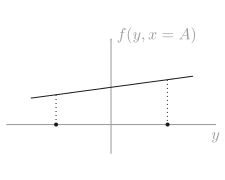
\includegraphics[width=8 cm]{inter1D.pdf}
\caption{Interpolación en la dirección $y$ sobre la línea 1-4.}
\label{fig:interp_1D}
\end{figure}

Usando una expresión análoga a la \cref{eq:interp_pol} se tiene la siguiente solución
\[f(x_A,y) = L_1(y)f_1 + L_4(y)f_4\, .\]
Procediendo de manera similar a lo largo de la línea 2-3 se obtiene
\[f(x_B,y) = L_2(y)f_2 + L_3(y)f_3\, .\]

Ahora nos encontramos en la posición de hacer la interpolación en la dirección 
$x$ usando las aproximaciones $f(x_A,y)$ y $f(x_B,y)$ previamente calculadas, 
escribiendo
\begin{align*}
  f(x,y) &= L_A(x) f(x_A,y) + L_B(x)f(x_B,y)\\
    &= L_A(x)[L_1(y)f_1 + L_4(y)f_4] + L_B(x)[L_2(y)f_2 + L_3(y)f_3]\\
    &= L_A(x)L_1(y)f_1 + L_A(x)L_4(y)f_4 + L_B(x)L_2(y)f_2 + L_B(x)L_3(y)f_3 \, 
    ,
\end{align*}
donde
\begin{align*}
L_A(x) & \equiv L_1(x)\, ,
&L_B(x) & \equiv L_2(x)\, ,\\
L_1(y) & \equiv L_1(y)\, ,
&L_2(y) & \equiv L_1(y)\, ,\\
L_3(y) & \equiv L_2(y)\, ,
& L_4(y) & \equiv L_2(x) \, .
\end{align*}

Los polinomios interpolantes que capturen simultáneamente la contribución en $x$ y en $y$ de cada valor conocido de la función  se forman entonces a partir de productos de polinomios de interpolación unidimensionales dando lugar al siguiente esquema de interpolación
\[f(x,y) = N_1(x,y)f_1 + N_2(x,y)f_2 + N_3(x,y)f_3 + N_4(x,y)f_4\, ,\]
en el cual los polinomios de interpolación $N_i(x,y)$ se definen como

\begin{align*}
N_1(x,y) & = L_1(x)L_1(y)\, ,
&N_2(x,y) & = L_2(x)L_1(y)\, ,\\
N_3(x,y) & = L_2(x)L_2(y)\, ,
&N_4(x,y) & = L_1(x)L_2(y)\, ,
\end{align*}
o, de forma explícita,
\begin{align*}
N_1(x, y) = \frac{1}{4}(1 - x)(1 - y)\, ,\\
N_2(x, y) = \frac{1}{4}(1 + x)(1 - y)\, ,\\
N_3(x, y) = \frac{1}{4}(1 + x)(1 + y)\, ,\\
N_4(x, y) = \frac{1}{4}(1 - x)(1 + y)\, .
\end{align*}


La \cref{fig:interp_4-nodos} muestra los 4 polinomios resultantes que satisfacen la propiedad 
\[N_i (x^j, y^j) = \begin{cases}
1,\quad \text{si } i = j\, ,\\
0,\quad \text{si } i \neq j\, .
\end{cases}\]

\begin{tcolorbox}
En el contexto del método de los elementos finitos para resolver problemas de elasticidad un elemento esta representado por un grupo de nudos, un conjunto de funciones de interpolación del tipo $N_i(x, y)$ correspondientes a cada nudo y estas se usan para aproximar el vector de desplazamientos en cualquier punto del elemento.
\end{tcolorbox}

\begin{figure}[H]
  \centering
  \includegraphics[width=5 in]{interp_4-nodos.pdf}
  \caption{Polinomios de interpolación para un dominio bidimensional con 4 puntos de muestreo.}
  \label{fig:interp_4-nodos}
\end{figure}

\newpage
\subsubsection{Ejercicios}
\begin{enumerate}
	
	\item \label{ejer:inter1} Considere la función $f(x) = x^5 + 4x^3 - 8$ y realice una interpolación de 
	orden 2. Introduzca ahora puntos adicionales de muestreo  para tratar de 
	mejorar la aproximación a la función. Compare los resultados gráficamente 
	mostrando la función exacta, los valores en los puntos de muestreo y el 
	polinomio de aproximación resultante. Realice también la comparación para la 
	primera derivada de la función.
	
	\item \label{ejer:inter2}
	Considere nuevamente la función $f(x) = {x^3} + 4{x^2} - 10$. Genere una tabla análoga a la \cref{tab:subdominio} pero esta vez con al menos 4 sub-dominios cada uno de 3 puntos de muestreo para el intervalo $[-1.0, 1.0]$. Usando lo puntos generados resolver el problema por medio de interpolación local de orden 2. Presentar gráficamente los polinomios interpolantes en los sub-dominios así como la correspondiente función de interpolación. Comparar esta ultima con la definición exacta de la función. Adicionalmente, calcular la primera derivada a partir de la definición exacta de la función y del polinomio de interpolación.
	
\item \label{ejer:inter3}
	Aproximar la función de Runge dada por:
	\[f(x) = \frac{1}{1 + 25x^2}\]
	mediante un esquema local o por tramos usando sub-dominios definidos por pares de puntos. Realizar tramos de longitud constante $\Delta x = 0.2$ y tramos de longitud variable con tamaños menores concentrados en los extremos y aumentando hacia el centro.
	
	
\end{enumerate}


\section{Integración numérica}
En diferentes aplicaciones de ingeniería y física es frecuente encontrarse con la necesidad de calcular numéricamente la integral de una función, ya sea que 
esta se tiene definida de manera explícita y su antiderivada no lo es, o en el caso de datos experimentales, cuando la función se encuentra definida de manera 
discreta.  En esta sección revisaremos algunas técnicas simples para abordar el problema de integración numérica de funciones. Inicialmente se revisará (a manera de repaso) la regla extendida del trapecio, la cual es  útil en el caso de funciones definidas. Posteriormente se considerará el caso de una función definida en términos de datos experimentales. Ambos problemas se abordarán para el caso de funciones de una sola variable y posteriormente estos métodos se extenderán al caso de dominios de integración bidimensionales. En la última parte de la sección se abordarán las denominadas formulas Gaussianas, las cuales resultan ser altamente poderosas y versátiles. Estas últimas son de uso común en métodos de elementos finitos y de elementos de frontera.

\subsection{Planteamiento del problema}
En el caso mas general estamos interesados en calcular numericamente integrales de la forma general

\begin{equation}
I\;=\iiint f(x,y,z)dV
\label{sample integral 2}
\end{equation}

donde la integral triple representa integración sobre un volumen determiando. De manera analoga al problema de interpolación, el problema de integración numérica también se resuelve a partir de la solución fundamental de integrar una función uni-dimensional. En cualquier caso, el problema de integración numérica se resuelve mediante una aproximación de la integral en términos de una suma ponderada de la forma:

\begin{equation}
\int\limits_a^b f(x) \dd{x}  \approx \sum\limits_{i=1}^n w_i f(x_i)\, ,
\label{eq:quadra}
\end{equation}

A estas formulas se les denomina {\bf cuadraturas}. En general en una cuadratura (o esquema de integración numérica) se evalúa la función $f(x)$ en $n$ puntos de coordenadas $x_i$ y cada valor de la función es ponderado por un factor $w_i$.


Por ejemplo la \cref{tab:ejemplo} muestra las abscisas (puntos de evaluación) y factores de ponderación de una cuadratura en particular. 

\begin{center}
	\begin{tabular}{cc}
		\hline
		$x_i$ & $w_i$ \\
		\hline
		$-0.86113$  & $0.34785$  \\
		$-0.33998$  & $0.65214$  \\
		$ +0.33998$  & $0.65214$  \\
		$ +0.86113$  & $0.34785$  \\
		\hline
	\end{tabular}
	\captionof{table}{Abscisas y factores de ponderación para calcular 
		$\int\limits_{-1}^{+1} f(x) \dd{x}$.}
	\label{tab:ejemplo}
\end{center}

Usando dicha cuadratura evaluaremos la integral 

\[I = \int\limits_{ - 1}^{ + 1} {({x^3} + 4{x^2} - 10)dx}\]

%\begin{equation}
%I = \int\limits_{ - 1}^{ + 1} {({x^3} + 4{x^2} - 10)dx}
%\label{eq:eje}
%\end{equation} 

La evaluación numérica de la integral se reduce entonces a calcular la siguiente suma ponderada:

\begin{align*}
\int\limits_{-1}^{+1} (x^3 + 4 x^2 - 10) \dd{x} \approx 0.34785 \cdot f(-0.86113) + 0.65214 \cdot f(-0.33998) \\
+ 0.34785 \cdot f(0.86113) + 0.65214 \cdot f(0.33998) = -17.3333
\end{align*}


\paragraph*{Ejemplo: Una aplicación en ingeniería civil.}
Supongamos que queremos calcular el área superficial del Valle de Aburrá. Aunque no conocemos una función que describa la topografía del valle de forma analítica, podemos representar la misma como una serie de puntos con coordenadas (latitud, longitud,  altitud) como se presenta en la siguiente figura.
\begin{figure}[H]
	\centering
	\includegraphics[width=10cm]{valle_aburra.png}
	\caption{Topografía del Valle de Aburrá.}
\end{figure}

Podemos utilizar las técnicas de interpolación vistas anteriormente para calcular la integral de superficie en el valle. Con la siguiente fórmula podríamos calcular el área superficial

\[A = \int\limits_\text{Dominio}{\sqrt{\left(\pdv{f(x, y)}{x}\right)^2 + 
\left(\pdv{f(x, y)}{y}\right)^2 + 1}}\; \dd{x}\dd{y}\, ,\]

en donde las coordenadas \((x, y)\) se corresponden con (longitud, latitud),  
la función \(f(x, y)\) es la altitud para cada uno de los puntos, y la integral 
se hace sobre el dominio sobre el que está definida la superficie.


\subsection{Integración numérica mediante polinomios de interpolación}

La integración numérica se basa fundamentalmente en el ajuste de un polinomio 
de interpolación $p(x)$ a la función dada $f(x)$ a través de $n$ puntos en 
los cuales se conoce o calcula el valor de la función, para luego usar 
$\int_a^b p(x)\dd{x}$ como una aproximación a la integral de $f(x)$. El número 
de evaluaciones de $f(x)$, así como las posiciones de los puntos de evaluación 
determinan que tan buena es la aproximación de $p(x)$ a $f(x)$ y por ende el 
error en la aproximación de la integral.

Concretamente, en los algoritmos de integración numérica se hace la aproximación:
\[\int\limits_a^b f(x) \dd{x} \approx \int\limits_a^b p(x) \dd{x}\, , \]
donde 
\[p(x) = \sum_{i=1}^n L_i(x) f(x_i)\]
siendo ${L_i}(x)$ el polinomio interpolante de Lagrange asociado al punto $x_i$.

Aproximando la función mediante un polinomio de interpolación se tiene que:
\[\int\limits_a^b f(x) \dd{x}  \approx \int\limits_a^b \sum_{i=1}^n 
L_i(x)f(x_i) \dd{x}  
\equiv \sum_{i=1}^n f(x_i)\int\limits_a^b L_i(x) \dd{x} \, , \]
la cual es equivalente a la \cref{eq:quadra} y en la cual se identifica que los 
factores de ponderación están dados por:
\begin{equation}
w_i \equiv \int\limits_a^b L_i(x) \dd{x} \, . 
\label{eq:pesos}
\end{equation}

Este tipo de esquemas se divide en métodos de Newton-Cotes y en cuadraturas 
Gaussianas. En el primer caso el intervalo de integración se divide en $n - 1$ 
sub-intervalos iguales (delimitados por abscisas equidistantes) de tamaño 
$(b-a)/(n - 1)$. En el segundo caso se dejan como parámetro de ajuste tanto la 
localización de los puntos de evaluación como los factores de ponderación, 
resultando en un esquema más versátil. A continuación se discuten ambas 
estrategias.


\subsection{Regla del trapecio}
Considere el caso particular en el que se tienen 2 puntos (1 intervalo de 
integración). El tamaño del intervalo en este caso corresponde a 
$h = b - a$ y el polinomio de interpolación de $f(x)$ está dado por:
\[p(x) = L_1(x) f_1 + L_2(x) f_2 \equiv L_1(x) f(a) + L_2(x) f(b)\, .\]

Los polinomios interpolantes en este caso son:
\begin{align*}
  &L_1(x) = \frac{(x - x_2)}{(x_1 - x_2)} \equiv  - \frac{1}{h}(x - b)\, \\
  &L_2(x) = \frac{(x - x_0)}{(x_2 - x_1)} \equiv \frac{1}{h}(x - a)\, .
\end{align*}

Reemplazando en \eqref{eq:pesos} se tiene que:
\begin{align*}
  &w_1 =  - \frac{1}{h}\int\limits_a^b (x - b) \dd{x}  \equiv \frac{h}{2}\, ,\\
  &w_2 =  + \frac{1}{h}\int\limits_a^b (x - a) \dd{x}  \equiv \frac{h}{2}\, ,
\end{align*}
de donde:
\[I = w_1 f_1 + w_2 f_2 \equiv \frac{h}{2}\left[f(a) + f(b)\right]\, .\]

Y, finalmente,
\begin{equation}
  \int\limits_a^b f(x) \dd{x} \approx \frac{h}{2}[ f(a) + f(b)]\, .
  \label{eq:trapecio}
\end{equation}

\subsubsection*{Ejemplo}
Calcular
\[I=\int\limits_{-1}^{+1} (x^3 + 4 x^2 - 10) \dd{x}\, ,\]
usando la regla del trapecio.

En este caso \(h=2.0\), luego:
\[I = f(-1) + f(1) \equiv  -7 - 5 = -12\]

Considere nuevamente la regla del trapecio dada en la \cref{eq:trapecio}. 
Supongamos un intervalo de integración con límites $x_1 = a$ y $x_n = b$ 
y en el cual se conocen en total $n$ valores de una función $f(x)$ (ver 
\cref{fig:test})
\begin{figure}[H]
\centering
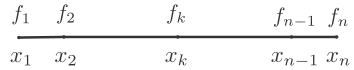
\includegraphics[width=10cm]{testline.pdf}
\caption{Intervalo de integración extendido con puntos de muestreo entre $x_1$ 
y $x_n$.}
\label{fig:test}
\end{figure}

Aplicando la \cref{eq:trapecio} $n - 1$ veces para hacer la integración en los 
sub-intervalos $(x_1, x_2),\, (x_2,x_3),\cdots,\, (x_{n-1},x_{n})$ y sumando 
los resultados se obtiene:
\begin{equation}
\int\limits_a^b f(x) \dd{x} = h\left[\frac{1}{2}f_1 + f_2 + f_3 + f_4 + \cdots 
+ f_{n-1} + \frac{1}{2}f_n \right]  + O\left[\frac{(b - a)^3 f''}{n^2} \right]
\label{eq:trap_comp}
\end{equation}
la cual es válida para calcular la integral usando los $n$ puntos $x_1,\, 
x_2,\cdots, x_{n- 1 }, x_{n}$. En esta expresión $h$ es la separación entre 
puntos.

En el apendice se describe la función {\bf trapz} (correspondiente a la 
\cref{eq:trap_comp}) la cual integra una función {\bf $f(x)$} entre los puntos $a$ y $b$. La 
rutina realiza la transformación del rango $[a,b]$ al ficticio dado por $[-1, 
+1]$. Usando esta función en el calculo de la integral del ejemplo antrior se tiene la siguiente salida:

\begin{verbatim}
Approximation for 1 subdivisions: -12.000000
Approximation for 2 subdivisions: -16.000000
Approximation for 3 subdivisions: -16.740741
Approximation for 4 subdivisions: -17.000000
Approximation for 5 subdivisions: -17.120000
Approximation for 6 subdivisions: -17.185185
Approximation for 7 subdivisions: -17.224490
Approximation for 8 subdivisions: -17.250000
Approximation for 9 subdivisions: -17.267490
Analytic integral: -17.333333
\end{verbatim}

\begin{tcolorbox}
En las cuadraturas de Newton-Cotes, como la regla del trapecio, los puntos de evaluación de la función son equidistantes. En las cuadraturas Gaussianas los puntos de evaluación no son equidistantes sino que estan localizados en ciertas posiciones de manera que la cuadratura sea lo mas eficiente posible.
\end{tcolorbox}



\subsection{Cuadraturas Gaussianas}
En la cuadratura correspondiente a la regla extendida del trapecio escrita de la forma
\begin{equation}
\int\limits_a^b f(x) \dd{x} \approx \sum\limits_{i=1}^{n} w_i f(x_i)\, ,
\label{quadra2}
\end{equation}
los puntos de evaluación se encuentran espaciados de manera equidistante. En 
las cuadraturas Gaussianas se dejan como parámetros por ajustar los factores de 
ponderación $w_i$ y también la localización de los puntos de evaluación $x_i$. 
Como resultado, ahora se dispone de $2n$ parámetros para ajustar y
así resolver el problema de calcular la integral de $f(x)$ entre $x=a$ y $x=b$ 
con la máxima precisión y el mínimo número de operaciones. Este 
tipo de cuadraturas proveen mayor precisión que las del tipo Newton-Cotes (como 
las del trapecio) cuando la función a integrar es apropiadamente representable 
mediante un polinomio. Considerando lo anterior se tiene que por medio de una 
cuadratura Gaussiana es posible integrar funciones expresables como:
\[\int\limits_a^b w(x) f(x) \dd{x}  \approx \sum\limits_{I = 1}^{n} w_i 
f(x_i)\, . \]

La factorización \(w(x) f(x)\) es útil ya que permite expresar una función como 
el producto de un polinomio $f(x)$ por una función conocida $w(x)$. Esta última 
puede seleccionarse para remover singularidades integrables de la integral.

%Considere a manera de ejemplo la integral de Gauss-Chebyshev:
%\[\int\limits_{-1}^1 \frac{e^{-cx^2}}{\sqrt {1 - x^2}} \dd{x} \equiv 
%\int\limits_{-1}^1 \frac{1}{\sqrt{1 - x^2} } e^{ -cx^2}\dd{x}\]
%donde
%\[w(x) = \frac{1}{\sqrt{1 - x^2}}\]
%mientras que: 
%\[f(x) = e^{ -cx^2}\, .\]
%
%Haciendo
%\[g(x) = w(x)f(x)\]
%y
%\[v_i = \frac{w_i}{w(x_i)}\, ,\]
%se tiene que:
%\begin{equation}
%  \int\limits_{-1}^{+1} g(x)\dd{x}  \approx \sum\limits_{i = 1}^{n} v_i 
%  g(x_i)\, .
%  \label{eq:gauss}
%\end{equation}

Las diferentes cuadraturas Gaussianas se encuentran especificadas en 
términos de una tabla de valores de abscisas de los puntos de integración (o de 
evaluación de la función a integrar) y sus correspondientes factores de 
ponderación (también denominados pesos). Por ejemplo la \cref{tab:ejemplo2} 
presenta las abscisas y factores de ponderación para una cuadratura de 4 puntos.
\begin{center}
\begin{tabular}{cc}
  \hline
  $x_i$ & $w_i$ \\
  \hline 
  $-0.86113$  & $0.34785$  \\
  $-0.33998$  & $0.65214$  \\
  $ +0.33998$  & $0.65214$  \\
  $ +0.86113$  & $0.34785$  \\
  \hline
\end{tabular}
\captionof{table}{Abscisas y factores de ponderación para calcular 
$\int\limits_{-1}^{+1} f(x) \dd{x}$}
\label{tab:ejemplo2}
\end{center}

Para facilitar la codificación de las cuadraturas y permitir cálculos 
generales, es común considerar el intervalo de integración canónico 
$[-1.0,+1.0]$, por lo que es necesario transformar la integral (incluyendo la 
función, los límites y el diferencial) a dicho intervalo como se 
discute en la \cref{sec:isopar}. La \cref{fig:quagauss} esquematiza este 
intervalo y los correspondientes puntos de integración (denotados por los 
círculos blancos). En la siguiente sección se desarrolla un ejemplo completo de 
evaluación de una integral por medio de una cuadratura Gaussiana tras realizar 
la transformación al dominio canónico.
\begin{figure}[H]
\centering

\includegraphics[width=10cm]{quagauss.pdf}
\caption{Esquematización de una cuadratura Gaussiana en el intervalo canónico 
$[-1.0,1.0]$.}
\label{fig:quagauss}
\end{figure}


\begin{tcolorbox}
En las cuadraturas Gaussianas los puntos de evaluación se encuentran especificados en el intervalo $[-1.0 , 1.0]$ el cual se denomina el espacio canonico. Es común denotar el espacio canonico mediante la variable $r$, de manera que para integrar una función en el intervalo $x \in [a , b]$ primero es necesario transformas la función y el dominio de integración al intervalo canonico $r \in [-1.0, 1.0].$
\end{tcolorbox}


\paragraph*{Ejemplo de derivación de una cuadratura Gaussiana.}
Revisemos el proceso de derivación de una cuadratura Gaussiana. Para esto supongamos que queremos formular una cuadratura correspondiente a $n=2$, o equivalentemente una cuadratura de 2 puntos , asumiendo que el intervalo de integración es $[a,b]=[-1,+1]$ de tal forma que coincida con el del intervalo canonico. Queremos entonces determinar los valores de los factores de ponderación $w_1$ y $w_2$ así como la localización de los puntos de evaluación $x_1$ y $x_2$ de manera que la cuadratura podamos integrar de manera exacta una función correspondiente a un polinomio de grado $3$ que tiene la forma general:

\[f(x) = a_0 + a_1 x + a_2 x^2 + a_3 x^3\, .\]

En otras palabras, queremos encontrar valores apropiados de $w_1$, $w_2$, $x_1$ y $x_2$ tales que se satisfaga:

\[I = \int\limits_{-1}^{+1} f(x)\dd{x}  \equiv w_1 f(x_1) + w_2 f(x_2)\, .\]

Usando $f(x)$ en $I$ y planteando la integral para cada termino se obtiene:
\[I = \int\limits_{-1}^{+1} a_0 \dd{x}  + \int\limits_{-1}^{+1} a_1 x\dd{x}  + \int\limits_{-1}^{+1} a_2 x^2 \dd{x}  + \int\limits_{-1}^{+1} a_3 x^3 \dd{x} \]

donde identificamos un término constante, un término de orden 1, un término cuadratico y un término de orden3. Para que la cuadratura sea exacta cada uno de estos términos debe poder ser integrado de manera exacta. Usando esta condición se tiene:

\begin{align*}
  &\intL_{-1}^{+1} \dd{x}  = 2 = w_1 \cdot 1 + w_2 \cdot 1\, ,\\
  &\intL_{-1}^{+1} x\dd{x}  = 0 = w_1 \cdot x_1 + w_2 \cdot x_2\, ,\\
  &\intL_{-1}^{+1} x^2 \dd{x}  = \frac{2}{3} = w_1 \cdot x_1^2 + w_2 \cdot 
  x_2^2\, ,\\
  &\intL_{-1}^{+1} x^3 \dd{x}  = 0 = w_1 \cdot x_1^3 + w_2 \cdot x_2^3\, .
\end{align*}


Se tiene un sistema de  ecuaciones en 4 incognitas correspondientes a los factores de ponderación $w_1$, $w_2$ y los puntos de evaluación $x_1$ y $x_2$. Resolviendo el sistema se tiene que $w_1 = 1$, 
$w_2 = 1$, $x_1 =-\sqrt{3}/3$ y $x_2 =  + \sqrt{3}/3$. Usando este resultado en la expresón de la cuadratura $I$ se tiene:

\[I = \int\limits_{-1}^{+1} f(x) \dd{x}  \approx 1.0 \cdot f(-\sqrt{3}/3) + 1.0 
\cdot f(+\sqrt{3}/3).\]

Claramente esta cuadratura es exacta si se trata de integrar funciones polinómicas de orden 3 o menor. Notese que la posibilidad de ajustar 4 paramétros $(w_1, w_2, x_1, x_2)$ permitió integrar de manera exacta una función de orden $3$. Mas adelante se demostrará que una cuadratura Gaussiana de orden $n$ permite integrar de manera exacta funciones de orden $2n-1$. Notese también que la localización de los puntos de integración $x_1$ y $x_2$ es simetrica con respecto a $x=0$: Mas aún, en este caso se satisface que $x_1 = - x_2$.

La idea de la cuadratura Gaussiana es extendible a polinomios de grado mayor, 
pero se requiere de un método efectivo para determinar los factores de
ponderación y abscisas de evaluación. En la siguiente sección se presentará un 
método aplicable a polinomios de orden $2n$, en el que se saca provecho de la 
propiedad de ortogonalidad de ciertos polinomios especiales.

\paragraph*{Polinomios ortogonales}
Dos polinomios $P(x)$ y $Q(x)$ donde $P(x) \ne Q(x)$ son ortogonales si:

\[\int\limits_a^b {P(x)Q(x)} dx = 0.\]
Particularmente, los polinomios de Legendre definidos por
\[P_n(x) = \frac{1}{2^n n!}\dv[n]{x} [(x^2 - 1)^n]\]
y los cuales son solución a la ecuación:
\[(1 - {x^2}) y'' - 2x y' + n(n + 1)y = 0\]
en el intervalo $[-1,+1]$ satisfacen la siguiente condición de ortogonalidad
\[\int\limits_{ - 1}^{ + 1} {{Q_i}(x)} {P_j}(x)\dd{x} = 0\, ,\]
donde  ${{Q_i}(x)}$ es cualquier función polinomial de grado $i$ menor que $j$.

Además de la propiedad de ortogonalidad los polinomios de Legendre tiene raíces 
en el intervalo $(-1.0, 1.0)$ las cuales son diferentes y simétricas con 
respecto a cero. Como se demuestra en el siguiente teorema esta ultima propiedad hace que estas raíces puedan ser útiles 
para producir una cuadratura que sea exacta para integrar cualquier función 
polinomial de grado menor que $2n$. Por ejemplo, el segundo polinomio de 
Legendre dado por:
\[{P_2}(x) = {x^2} - \frac{1}{3}\]
tiene como raíces $x_1 =  - \frac{\sqrt{3}}{3}$ y $x_2 =  +\frac{\sqrt{3}}{3}$ 
los cuales corresponden a los puntos de integración para la cuadratura
exacta de grado 3 encontrada en el ejemplo anterior.

\paragraph*{Teorema}
Sean $\left\{ x_1, x_2,\cdots, x_n \right\}$ las raíces del polinomio de 
Legendre $P_n(x)$ de grado $n$; sea
\[w_i = \int\limits_{-1}^{+1} \prod\limits_{j=1}^n \frac{x - x_j}{x_i - x_j} 
\dd{x}\, , \]
y sea $f(x)$ una función polinomial cualquiera de grado menor que $2n$, entonces:
\begin{equation}
  I = \int\limits_{-1}^{+1} f(x)\dd{x}  = \sum\limits_{i=1}^n w_i f(x_i)\, .
  \label{eq:Legendre}
\end{equation}


\paragraph*{Demostración}

\begin{enumerate}
\item Si $f(x)$ es de grado menor que $n$ entonces claramente es representable 
en términos de polinomios de Lagrange con lo cual se satisface de manera 
automática la condición \cref{eq:Legendre}.

\item Si $f(x)$ es de grado menor que $2n$ entonces es representable como:
\[f(x) = Q(x){P_n}(x) + R(x)\]
donde $Q(x)$ es el cociente de $f(x)/{P_n}(x)$ y de grado $n-1$ (o menor) y $R(x)$ es el residuo y de grado menor que $n$. Integrando esta representación de $f(x)$ se tiene:
\[\int\limits_{-1}^{+1} Q(x) P_n(x) \dd{x}  + \int\limits_{-1}^{+1} R(x) \dd{x}\, , \]
la cual se reduce a:
\[I = \int\limits_{ -1}^{ +1} f(x) \dd{x}  = \int\limits_{ -1}^{ +1} R(x)\ \dd{x}\, , \]
tras usar la propiedad de ortogonalidad entre $Q(x)$ y $P_n (x)$. Ahora, retomando la expresión:
\[f(x) = Q(x){P_n}(x) + R(x)\]
si esta es evaluada en las raíces de los polinomios de Legendre se tiene que:
\[f(x_i) = R(x_i)\]
con lo cual queda completa la demostración.

\end{enumerate}

\subsection{Transformación del dominio de solución}\label{sec:isopar}
La construcción de tablas con las coordenadas y factores de ponderación de las diferentes cuadraturas y su programación en el computador se facilita si estas se especifican para un rango fijo. Por diversas conveniencias matemáticas, es común usar como 
intervalo general el dado por $[-1, 1]$ denominado previamente como el intervalo canonico y descrito mediante una variable independiente, comunmente denotada como $r$. Se tiene entonces que el espacio de la variable independiente correspondiente a $x \in [a , b]$ se transforma el espacio canonico dado por $r \in [-1.0 , 1.0]$. Note que esta transformación también implica una transformación de la función $f(x)$ en el espacio de $x$ a su respresentación en el espacio de $r$.

Es necesario entonces reescribir la integral de $f(x)$ en el rango comprendido entre $x=a$ y $x=b$ a una integral en el espacio canonico de acuerdo con:
\begin{equation}
\int\limits_a^b f(x) \dd{x} \equiv \int\limits_{-1}^{+1} F(r) \dd{r}\, . 
\label{eq:trans}
\end{equation}


La transformación \ref{eq:trans} se describe en la \cref{fig:map} y en la cual la flecha curva esquematiza la transformación entre los 2 espacios a saber, el espacio representado mediante la variable independiente $x$ y 
comprendido entre $x=a$ y $x=b$ y el espacio canonico descrito mediante la variable  $r$ y comprendido entre $r=-1$ y  $r=1$.

\begin{figure}[H]
\centering
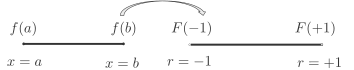
\includegraphics[width=10cm]{transformacion.pdf}
\caption{Transformación del rango de integración $[a,b]$ al intervalo canónico 
$[-1.0,+1.0].$}
\label{fig:map}
\end{figure}

La transformación espacial puede indicarse matemáticamente como:
\begin{align*}
  x = x(r)\, ,
  r = r(x)\, ,
\end{align*}
y en la cual $x(r)$ y $r(x)$ denotan relaciones funcionales entre los 2 espacios. Es evidente que independiente de la forma de la relación funcional esta minimamente debe satisfacer las condiciones $x(-1.0)=a$ y $x(+1)=b$. Por ejemplo, una relación relación funcional válida puede encontrarse tras asumir que ambos espacios están relacionados mediante un polinomio de interpolación de Lagrange de primer grado construido como:

\[x(r) = L_1(r) x(r_1) + L_2(r) x(r_2)\, .\]

Usando los correspondientes polinomios interpolantes:

\begin{align*}
  &L_1(r) = \frac{r - r_2}{r_1 - r_2} \equiv \frac{1}{2}(1 - r)\, ,\\
  &L_2(r) = \frac{r - r_1}{r_2 - r_1} \equiv \frac{1}{2}(1 + r)\, ,
\end{align*}

en la expresión para $x(r)$ se tiene que:

\[x(r) = \frac{1}{2}(a + b) + \frac{r}{2}(b - a).\]

Continuando con la transformación es claro que también es necesario reescribir $f(x)$ en términos de  $r$  de acuerdo con:

\[f = f(x) \equiv f[x(r)] = \hat F(r)\, .\]

Finalmente, para completar la transformación es necesario transformar el diferencial de "espacio físico", es decir $dx$ a su correspondente diferencial en el espacio canonico $dr$. Procediendo directamente desde la transformación en términos de los polinomios de Lagrange se tiene que:

\[\dv{x}{r}  = \dv{L_1(r)}{r} x(r_1) + \dv{L_2(r)}{r} x(r_2) \equiv 
\frac{1}{2}(b - a)\, ,\]

y por lo tanto

\[\dv{x}{r} = \frac{1}{2}(b - a)\]

lo cual permite escribir finalmente la integral en el dominio ficticio comprendido entre $[-1, +1]$ de acuerdo con:

\[\int\limits_a^b f(x) \dd{x} \equiv \int\limits_{-1}^{+1} \hat F(r)\frac{h}{2} 
\dd{r} \equiv \int\limits_{-1}^{+1} F(r) \dd{r}\, , \]

y donde $h = \frac{1}{2}(b - a).$

\subsubsection*{Ejemplo}

Usar una cuadratura Gaussiana de 2 puntos (ver \cref{ejemplo3}) para evaluar la integral:
\[I = \int\limits_0^3 (2^x - x) \dd{x}\, . \]

\begin{center}
\begin{tabular}{cc}
  \hline
  $x^I$ & $w^I$ \\
  \hline 
  $-0.5773503$  & $1.000000$  \\
  $+0.5773503$  & $1.000000$  \\
  \hline
\end{tabular}
\captionof{table}{Abscisas y factores de ponderación para calcular $\int_{-1}^{+1} f(r) \dd{r}$}
\label{ejemplo3}
\end{center}

Para realizar la integración usando la cuadratura Gaussiana de 2 puntos dada en la \cref{ejemplo3} es necesario transformar el rango de integración y el integrando de la función al espacio correspondiente al intervalo $[-1.0,+1.0]$. Esta transformación está dada por:
\[x(r) = \frac{3}{2} + \frac{3}{2}r\]
mientras que los elementos diferenciales satisfacen
\[\dd{x} = \frac{3}{2}\dd{r}\, .\]

Para transformar la función usamos
\[\hat f(r) = f[x(r)] \equiv f\left( \frac{3}{2} + \frac{3}{2}r \right)\, ,\]
de donde se tiene que
\[I = \int\limits_0^3 (2^x - x) \dd{x} = \int\limits_{-1.0}^{+1.0} \left[ 2^{\frac{3}{2}(1 + r)} - \frac{3}{2}(1 + r) \right] \frac{3}{2} \dd{r} \, ,\]
y evaluando,
\begin{align*}
  I &= \sum\limits_{i=1}^2 w_i\left[ 2^{\frac{3}{2}(1 + r_i)} - \frac{3}{2}(1 + 
  r_i) \right]\frac{3}{2}\\
  &= 1.0 \cdot (1.37678967978) + 1.0 \cdot (4.18374583924)\\
  &= 5.56053551
\end{align*}

En el apendice se presenta a manera de función la implementación en Python de la cuadratura Gaussiana de 2 puntos. La rutina hace uso  de la función {\bf gauss1d} para integrar la función definida en {\bf $f(x)$}. La rutina realiza la transformación de $[a,b]$ a $[-1, +1]$.

%\pagebreak
%\begin{minted}[mathescape,
%	gobble=4,
%	frame=lines,
%	framesep=2mm]{python} 
%    import numpy as np
%    from scipy.special import roots_legendre # Gauss points and weights
%    from sympy import symbols, integrate
%    
%    
%    def gauss1d(fun, x0, x1, n):
%    """Gauss quadrature in 1D
%    
%    Parameters
%    ----------
%    fun : callable
%        Function to integrate.
%    x0 : float
%        Initial point for the integration interval.
%    x1 : float
%        End point for the integration interval.
%    n : int
%        Number of points to take in the interval.
%    
%    Returns
%    -------
%    inte : float
%         Approximation of the integral
%    
%    """
%    xi, wi = roots_legendre(n)
%    inte = 0
%    h = 0.5 * (x1 - x0)
%    xm = 0.5 * (x0 + x1)
%    for cont in range(n):
%        inte = inte + h * fun(h * xi[cont] + xm) * wi[cont]
%    return inte
%
%    fun = lambda x: x**3 + 4*x**2 - 10
%    gauss_inte = gauss1d(fun, -1, 1, 4)
%    x  = symbols('x')
%    analytic_inte = integrate(fun(x) , (x , -1 , 1))
%    print("Analytic integral: {:.6f}".format(float(analytic_inte)))
%    print("Gauss quadrature: {:.6f}".format(gauss_inte))
%\end{minted}

Si ejecutamos la rutina, obtenemos el siguiente resultado:
\begin{verbatim}
Analytic integral: -17.333333
Gauss quadrature: -17.333333
\end{verbatim}

\subsection{Extensión a dominios en 2D}
En varias aplicaciones de ingeniería es necesario el calculo de integrales sobre dominios bi-dimensionales, posiblemente con geométrias arbitrarias. En esta sección se generaliza la idea de la cuadratura numérica presentada en los numerales anteriores para funciones de 1 sola variable independiente al caso de funciones de varias variables. En particular, acá ausmimos que las variables independientes representan coordenadas $x , y$ de un espacio cartesiano.

En la \cref{fig:rieman} se esquematiza un dominio en 2-dimensiones (línea negra continua) denotado como $R$ y sobre el cual se desea calcular una integral de la forma
\[I = \iint\limits_R f(x,y) \dd{A}\, . \]

Para proceder con el cálculo el dominio se ha dividido en $N$ subdominios 
rectangulares (líneas negras punteadas) de manera que un subdominio típico 
tiene dimensiones $\Delta {x_i} \times \Delta {y_i}$.

\begin{figure}[H]
\centering
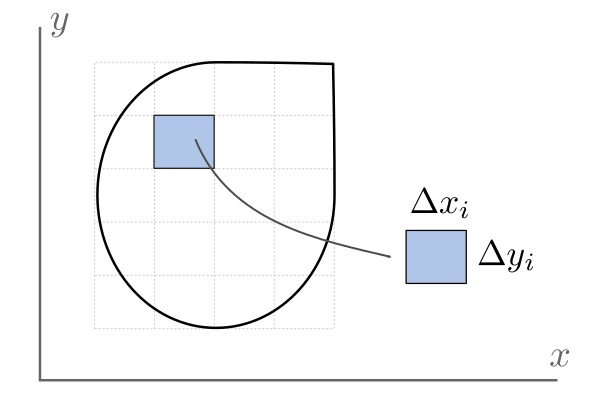
\includegraphics[width=10cm]{riemann.pdf}
\caption{Partición de Riemman para un dominio plano.}
\label{fig:rieman}
\end{figure}

Definiendo

\[p = \max\{ \Delta {x_i}, \Delta {y_i} \}\, ,\]

como la norma de la partición, se tiene, de acuerdo a la definición de una integral como una suma de Riemann, que:

\[I = \iint\limits_R  f(x,y) \dd{A}  \equiv \lim_{p \to 0} \sum_{j=1}^N f(x_j,y_j) \Delta x_j \Delta y_j\, .\]

Ahora, tomando cada uno de los límites en la dirección $x$ y $y$ por separado permite identificar 2 procesos de integración de tal forma que la integral sobre $R$ se reduce a la integral doble dada por:

\[I = \iint f(x,y) \dd{x}\dd{y}\, . \]

Para identificar los límites de integración considere la \cref{fig:dirx}. En esta se muestra un dominio de integración rectangular (en sombreado azul) cuyo lado mayor es paralelo a la dirección $x$ y con altura media correspondiente a un valor constante $y$. Los lados menores del rectángulo tienen abscisas $x_1(y)$ y $x_2(y)$ respectivamente.
\begin{figure}[H]
\centering
\includegraphics[width=8cm]{inte_dirx.pdf}
\caption{Integración en la dirección x.}
\label{fig:dirx}
\end{figure}

Claramente se tiene que para el valor de $y$ constante la contribución a la integral $I$ sobre la región $R$ del rectángulo acotado por ${x_1}(y)$ y ${x_2}(y)$ esta dada por:

\[\int\limits_{x_1(y)}^{x_2(y)} f(x,y) \dd{x}\, ,\]

de forma que el cálculo de la integral sobre la totalidad de la region $R$ se completa repitiendo el proceso para valores de $y$ constantes variando entre $y_1$ y $y_2$ y dando la integral total como:

\begin{equation}
  I = \int\limits_{y_1}^{y_2} \left\{ \int\limits_{x_1(y)}^{x_2(y)} f(x,y) \dd{x}  \right\} \dd{y}
  \label{iterada}
\end{equation}


Para dar mayor claridad a la \cref{iterada}, nótese que la integral interna puede escribirse como una función de $y$

\[F(y) = \int\limits_{x_1(y)}^{x_2(y)} f(x,y) \dd{x}\, , \]

y la integral externa como

\[I = \int\limits_{y_1}^{y_2} F(y) \dd{y}\, . \]

Notese que el calculo de $I$ se ha reducido a 2 integrales uni-dimensionales y en consecuencia el proceso puede resolverse por medio de las cuadraturas uni-dimensionales ya discutidas. En este caso la función mas interna $F(y)$ resulta de integrar solo la variación en $x$ y posteriormente la integral $I$ resulta de integrar la variación en $y$. Alternativamente (ver \cref{fig:diry}) también es posible definir

\[H(x) = \int\limits_{y_1(x)}^{y_2(x)} f(x,y) \dd{y} \]

de manera que la integral completa $I$ queda definida por

\[I = \int\limits_{x_1}^{x_2} H(x) \dd{x}. \]

\begin{figure}[H]
\centering
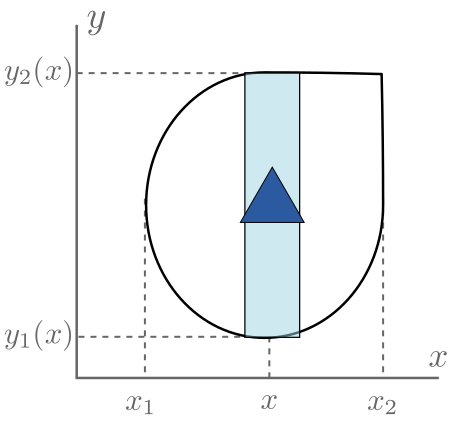
\includegraphics[width=8cm]{inte_diry.pdf}
\caption{Integración en la dirección y.}
\label{fig:diry}
\end{figure}


\subsubsection*{Ejemplo}

Considere la región (o dominio) triangular de la \cref{fig:ejeint}.


\begin{figure}[h]
	\centering
	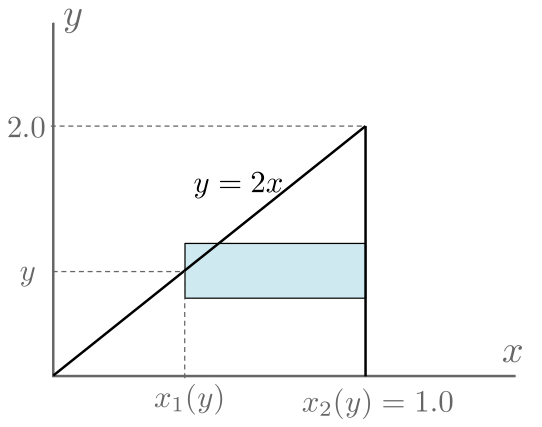
\includegraphics[width=8cm]{ejeint.pdf}
	\caption{Integración en la dirección x sobre la región triangular $R$.}
	\label{fig:ejeint}
\end{figure}



Utilice el concepto de integrales iteradas discutido anteriormente para determinar la integral de la función

\[f(x,y)=x y^2\]

sobre la región $R$ de la figura.

La integral sobre $R$ esta dada por

\[I = \iint f(x,y) \dd{A}\]

donde $dd{A}$ representa un elemento diferencial de superficie. Supongamos que tomaremos rectangulos paralelos al eje $x$ de manera que para valores constantes de $y$ se tiene:

\[x_1(y) = \frac{y}{2}\]
y
\[x_2(y) = 1\]

y por lo tanto se tiene que:
\[F(y) = \int\limits_{x_1(y)}^{1.0} x y^2 \dd{x}  \equiv \int\limits_{y/2}^{1.0} x y^2 \dd{x}\, , \]

luego

\[F(y) = \left[ \frac{1}{2} x^2 y^2 \right]_{y/2}^{1.0} \equiv \frac{1}{2} y^2 
- \frac{1}{8}  y^4\, .\]

Identificando ahora los limites inferior y superior en la dirección $y$ como ${y_1} = 0$ y ${y_2} = 2$ es posible integrar la dependencia en $y$ de acuerdo con:

\[I = \int\limits_0^{2.0} F(y) \dd{y}  \equiv \int\limits_0^{2.0} 
\left(\frac{1}{2}y^2 - \frac{1}{8} y^4\right) \dd{y}  \equiv \frac{8}{15}\, .\]


% respectivamente y las funciones ${{x_1}(y)}$ y ${{x_2}(y)}$  como:
%\[x_1(y) = \frac{y}{2}\]
%y
%\[x_2(y) = 1\]
%se tiene que:
%\[F(y) = \int\limits_{x_1(y)}^{1.0} x y^2 \dd{x}  \equiv \int\limits_{y/2}^{1.0} x y^2 \dd{x}\, , \]
%luego
%\[F(y) = \left[ \frac{1}{2} x^2 y^2 \right]_{y/2}^{1.0} \equiv \frac{1}{2} y^2 
%- \frac{1}{8}  y^4\, .\]
%Usando esta función para integrar en $y$ se llega a
%\[I = \int\limits_0^{2.0} F(y) \dd{y}  \equiv \int\limits_0^{2.0} 
%\left(\frac{1}{2}y^2 - \frac{1}{8} y^4\right) \dd{y}  \equiv \frac{8}{15}\, .\]

Procediendo de manera alternativa (ver \cref{fig:ejeinty}) es posible escribir:
\[H(x) = \int\limits_{y_1(x)}^{y_2(x)} x y^2 \dd{y} \]
y
\[I = \int\limits_{x_1}^{x_2} H(x) \dd{x}\, . \]

\begin{figure}[H]
\centering
\includegraphics[width=8cm]{ejeinty.pdf}
\caption{Integración en la dirección y sobre la región triangular $R$.}
\label{fig:ejeinty}
\end{figure}

donde:
\[{y_1}(x) = 0\]
\[{y_2}(x) = 2x\]
luego
\[H(x) = \int\limits_0^{2x} {x{y^2}dy}  \equiv \left. {\frac{1}{3}x{y^3}} \right|_0^{2x} \equiv \frac{8}{3}{x^4}\]
de manera que la integral se reduce a:
\[I = \int\limits_0^{1.0} {\frac{8}{3}{x^4}dx}  \equiv \frac{8}{{15}}.\]

En el apendice se presenta una rutina con la correspondiente implementación en Python del esquema de integrales iteradas. Esta permite calcular integrales sobre regiones rectangulares. Por ejemplo si se calcula la siguiente integral

\[\int\limits_0^2\int\limits_0^2 [3xy^2 - x^3] \dd{x}\dd{y} = 8\, , \]

usando la rutina código se obtiene el siguiente resultado:

\begin{verbatim}
Gauss quadrature: 8.000000
\end{verbatim}

\newpage
\subsubsection{Ejercicios}
\begin{enumerate}
%	
	\item \label{punto01} Calcule la integral de la función
	
	\[f(x,y)=4x^2+3xy+y^2\]
	
	sobre los dominios planos mostrados en las figuras
	
	
	\begin{figure}[H]
		\centering
		\includegraphics[width=0.65\textwidth]{domain1}
		\caption{Dominios de integración para el problema 1.}
		\label{fig:tan1}
	\end{figure}
	
	

	
	
	\item \label{punto02} Calcule la integral de la función
	
	\[f(r,s)=rs\]
	
	sobre el dominio triangular mostrado en la figura
	
	\begin{figure}[H]
		\centering
		\includegraphics[width=0.50\textwidth]{domain3}
		\caption{Dominios de integración para el problema 2.}
		\label{fig:tan2}
	\end{figure}
	
	\item \label{punto03} Calcular las siguientes integrales usando una cuadratura de Gauss apropiada:
	
	\[I=\int_{1.0}^{1.5}x^2\ln x\operatorname dx\]
	
	\[I=\int_0^\frac{\mathrm\pi}4e^{3x}Sin2x\operatorname dx\]
	
	\[I=\int_0^\frac{\mathrm\pi}4Cos^2x\operatorname dx\]

	
	
\end{enumerate}

